\label{sec:calibration}

This chapter describes the configuration in which the allocation question is
measurable at all. That is not a formality: most natural configurations of a
differentially private detector are uninformative, either because the noise
destroys the model or because it does not reach it, and in both cases every
schedule scores alike. Constructing a regime in which accuracy is genuinely
sensitive to the noise multiplier is a precondition for the results in
Chapter~5, and the procedure for finding it is a contribution in its own right.

\section{Dataset and Partitioning}

We use the Anti-UAV600 thermal infrared benchmark \cite{zhao20233rd}. Sequences
are grouped by \emph{recording session}, identified by the timestamp prefix:
clips sharing a prefix are the same recording seconds apart, so splitting them
across train and test leaks near-duplicate frames. We found this leak in an
earlier folder-level split, in which 5 of 11 evaluation sessions also appeared
in training, and eliminate it here. A second leak was found and removed in the
public pretraining pool, 4 of whose 20 folders shared a session with the
evaluation subset; the trunk is therefore re-pretrained on a session-disjoint
97-folder pool.

\vspace{10pt}

Experiments use a 29-sequence clear-sky subset spanning 17 sessions. On
cluttered sequences the detector saturates near $0.0$--$0.10$ mAP, and
degradation cannot be measured against a floor: every schedule scores alike.
Removing that floor effect is what makes the allocation question measurable. The
final split is $5\times3{,}808$ training frames across five clients and
$1{,}500$ evaluation frames, disjoint by session.

\vspace{10pt}

Restricting to clear-sky sequences raises absolute accuracy and is therefore a
favourable choice, but it favours the \emph{alternative} hypothesis rather than
ours: it is the condition under which a non-uniform schedule has the most room
to demonstrate an advantage. The negative result of Chapter~5 is obtained in the
setting most generous to the method it fails to support.

\section{Model: Public Trunk, Private Head}

The architecture follows from a tension established by direct measurement.
DP-training an entire detector destroys it, yielding $0.0$--$0.10$ mAP at every
usable noise level, while DP-training only a small $12{,}677$-parameter head on
frozen public features makes the noise irrelevant: we measured no effect at all
from $\sigma=0$ to $\sigma=512$, that is, from $\varepsilon=\infty$ down to
$\varepsilon\approx0.104$. The informative regime lies between these extremes.

\vspace{10pt}

We therefore pretrain a convolutional trunk on a session-disjoint public pool,
freeze and cache its first three stages $s_1$--$s_3$, and privately train the
two subsequent stages $k_1,k_2$ together with the detection head, giving
$D=566{,}789$ differentially private parameters. Note that $D$ is what is
\emph{privatised}, not what is randomly initialised; the distinction matters for
the initialisation choice below.

\vspace{10pt}

Two implementation details proved essential, and both are reported because
neither is obvious in advance.

\begin{itemize}
  \item \textbf{SGD, not Adam.} Under Adam a sixteen-fold change in $\sigma$
  produced no change in accuracy ($0.336$ against $0.320$), because
  per-coordinate normalisation rescales noise-dominated gradients to
  fixed-size steps. Under SGD the same noise gives monotone degradation
  ($0.311$, $0.311$, $0.247$ at $\sigma=0.5,2,8$). Adaptive optimisers make the
  privacy parameter inert, which is a silent failure: the privacy accountant
  still reports the intended $\varepsilon$ while the noise never reaches the
  weights. Figure~\ref{fig:adam} shows both panels.
  \item \textbf{Initialisation.} Training $k_1,k_2$ and the head from scratch
  collapses to all-background at every learning rate tried. Seeding $k_1,k_2$
  from the public trunk while leaving the head random keeps optimisation stable
  and preserves dynamic range, with a floor of $0.001$ and a no-DP ceiling of
  $0.769$ IoU$_{.25}$.
\end{itemize}

\begin{figure}[H]
\centering
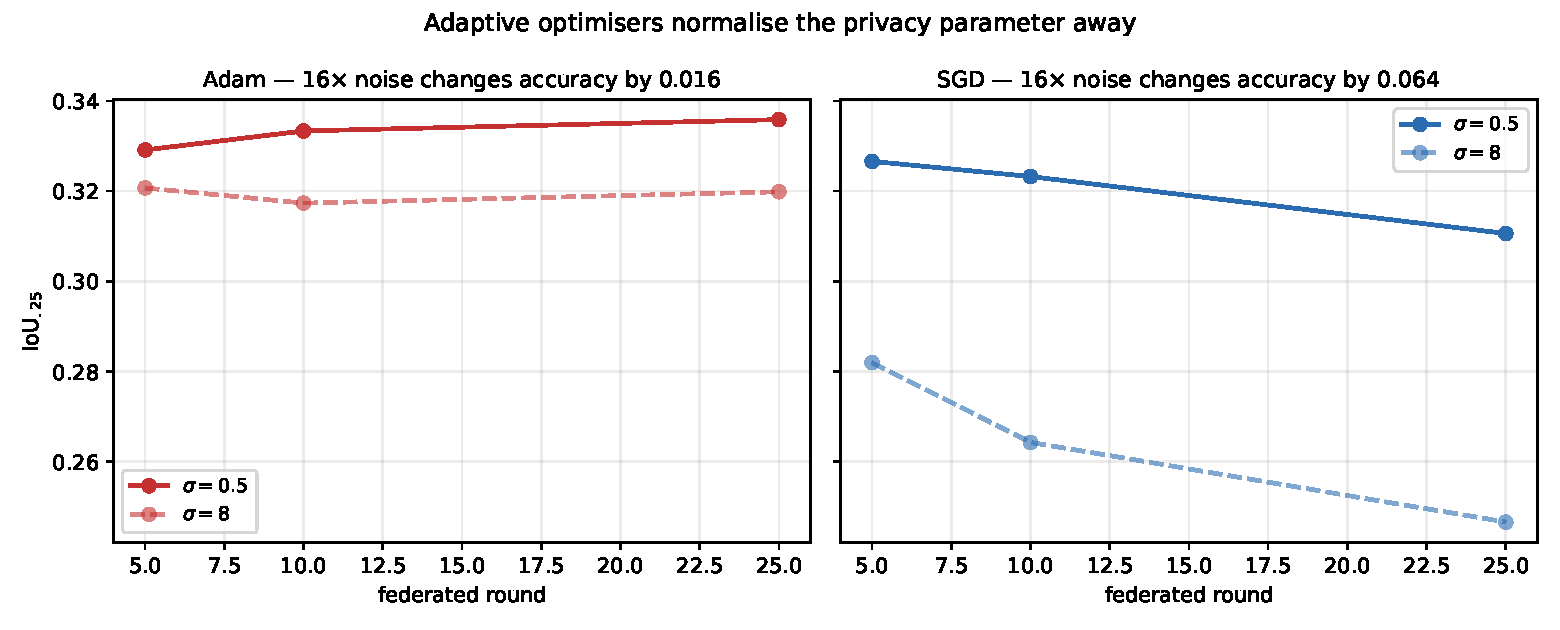
\includegraphics[width=\textwidth]{figF_adam_vs_sgd.pdf}
\caption{Adaptive optimisers normalise the privacy parameter away. A
sixteen-fold change in $\sigma$ moves final accuracy by $0.016$ under Adam and
$0.064$ under SGD, with the SGD degradation monotone in both noise and rounds.}
\label{fig:adam}
\end{figure}

\section{Locating the Informative Regime}

Effective signal-to-noise ratio per round scales as
\begin{equation}
  \text{eff.\ SNR} \;\propto\; \frac{B}{\sigma\sqrt{D}}\sqrt{\text{steps}\cdot N}
  \;\propto\; \frac{\sqrt{B}}{\sigma\sqrt{D}},
  \label{eq:snr}
\end{equation}
since the number of steps scales as $1/B$. Signal accumulates coherently across
steps and clients while noise accumulates as a square root, which is why the
averaging gain enters as $\sqrt{\text{steps}\cdot N}$.

\vspace{10pt}

Calibrating the constant on the head-only configuration, where the knee sits at
$\sigma\approx512$ for $D=12{,}677$ and $B=2048$, predicts a degradation knee at
$\sigma_{\text{knee}}\approx 1.69\sqrt{B}$ for $D=566{,}789$. The predictions of
$38$ at $B=512$ and $19$ at $B=128$ were borne out by measured onsets of
$32$--$64$ and $16$--$32$ respectively, so the model is accurate to within a
factor of two and is usable for choosing $B$ in advance rather than by sweeping.
We adopt $B=128$, SGD with learning rate $0.003$ and momentum $0.9$, $C=1$, and
$T=25$ rounds of $E=2$ local epochs.

\vspace{10pt}

Table~\ref{tab:noise} gives the resulting operating curve, and
Figure~\ref{fig:operating} plots it against the source method's operating range.
A trivial constant-output predictor scores $0.021$, confirming that the metric
is not degenerate; targets are well spread, with the most common cell occupied
in $4.6\%$ of frames.

\begin{table}[H]
\centering
\caption{Noise sensitivity in the calibrated regime. IoU$_{.25}$ on held-out
sessions; floor (random head) $0.001$, trivial predictor $0.021$.}
\label{tab:noise}
\begin{tabular}{lcccccc}
\toprule
$\sigma$ & 0 & 2 & 4 & 8 & 16 & 32 \\
\midrule
IoU$_{.25}$ & 0.769 & 0.557 & 0.499 & 0.492 & 0.371 & 0.047 \\
\bottomrule
\end{tabular}
\end{table}

\begin{figure}[H]
\centering
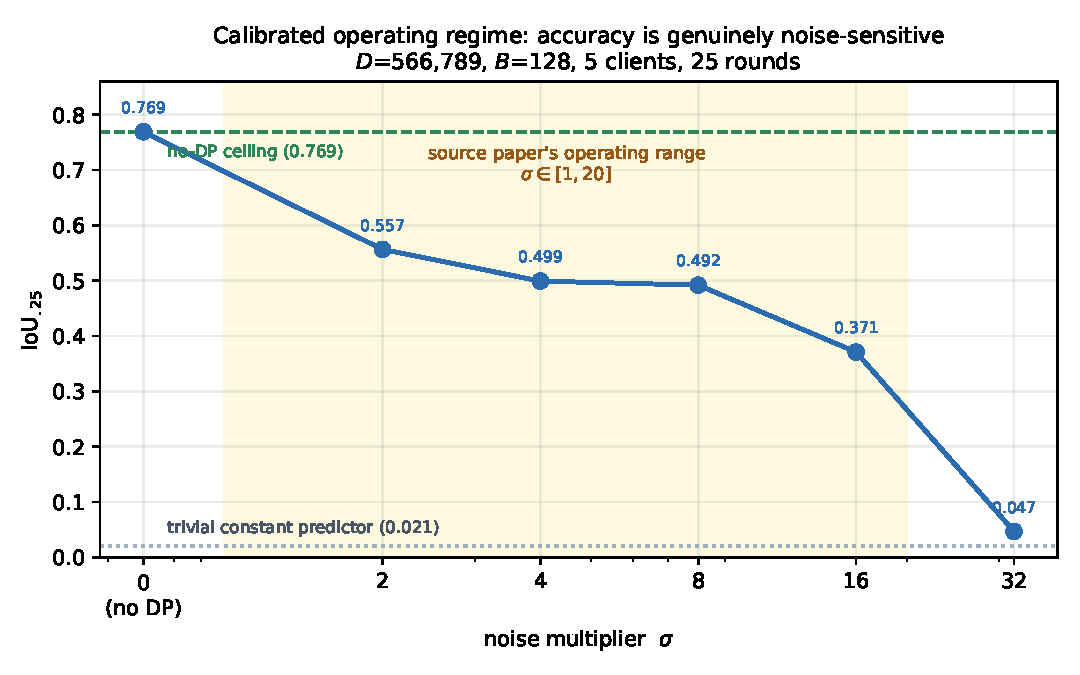
\includegraphics[width=0.85\textwidth]{figE_operating_curve.pdf}
\caption{The calibrated operating regime. Accuracy is genuinely sensitive to the
noise multiplier across the source method's operating range $\sigma\in[1,20]$,
which is the precondition for any allocation study. Floor and ceiling are
marked.}
\label{fig:operating}
\end{figure}

\section{Verifying the Theorem's Assumption}
\label{sec:clipbinds}

Theorem~\ref{thm:uniform} rests on assumption~(i): that per-sample clipping
binds, so each round's signal contribution is pinned at $C$. This is not an
idealisation to be taken on trust. It is measurable, and it is the single
quantity that determines whether adaptive allocation has anything to work with.
Table~\ref{tab:clipbinds} reports median per-sample gradient norms against the
clipping threshold, for our detector and for the small convolutional network and
$C=6$ used by the source method on CIFAR-10.

\begin{table}[H]
\centering
\caption{Does clipping bind? Median per-sample gradient norm against the
clipping threshold $C$. Clipping binds in both settings, so assumption~(i) of
Theorem~\ref{thm:uniform} holds for the source method's own configuration as
well as for ours.}
\label{tab:clipbinds}
\begin{tabular}{llrrr}
\toprule
Setting & Stage & Median $\lVert g_i\rVert$ & $C$ & Binds by \\
\midrule
CIFAR-10 CNN ($D=59{,}386$) & initialisation & 1.18 & 6.0 & --- \\
                            & after 5 rounds & 37.93 & 6.0 & $6.3\times$ \\
                            & after 25 rounds & 48.11 & 6.0 & $8.0\times$ \\
\midrule
Anti-UAV head ($D=566{,}789$) & steady state & 26.85 & 1.0 & $26.8\times$ \\
\bottomrule
\end{tabular}
\end{table}

Two observations follow. First, clipping binds in \emph{both} settings, by
$8\times$ on CIFAR-10 and $27\times$ on the detector, so the difference between
them is one of degree rather than of regime, and the optimality result applies
to both. At initialisation the CIFAR-10 gradients sit below the threshold and no
clipping occurs, but the fraction of clipped samples rises to $0.90$ within five
rounds and remains high thereafter, so the binding regime is reached almost
immediately and holds for all but the opening rounds.

\vspace{10pt}

Second, and more directly damaging to the motivating intuition, the per-sample
gradient norm \emph{grows} over training on CIFAR-10, from $1.18$ at
initialisation to $48.11$ after 25 rounds. The adaptive-allocation argument
assumes the opposite, that gradients are large early and shrink as the model
converges, so that noise should be front-loaded. Under cross-entropy on a small
network the per-sample gradient norm increases with training as the model grows
confident and the loss surface sharpens, and in any case clipping removes the
variation before it can reach the aggregate. The premise is therefore doubly
unavailable: the quantity it relies on moves the wrong way, and is then
discarded by the mechanism.

\section{Threat Model for the Poisoning Study}

The aggregation server is honest but curious: it follows the protocol and does
not inject updates of its own, but may inspect what it receives, which is the
motivation for client-side DP. Up to $30\%$ of clients are malicious and may
submit arbitrary updates. Malicious clients know the global model, the detection
rule in force and the DP parameters, which is the strongest information
assumption under which a norm-preserving attack is meaningful. They cannot
observe honest clients' private data or the server's held-out validation set.
Section~\ref{sec:p3-envelope} derives what this threat model permits an attacker
to do, and the answer constrains the attacks worth implementing.

\section{Statistical Protocol}
\label{sec:protocol}

Comparisons are \emph{paired}: all schedules within a trial share one
initialisation and one random-number stream, a common-random-numbers (CRN)
design, so the noise draws are correlated across arms and initialisation luck
cancels. CRN reduced the standard deviation of paired differences from $0.0466$
to $0.0171$, a $3.2\times$ tightening, so that 20 paired trials carry the
precision of roughly 150 without it. Scores are the mean IoU$_{.25}$ over the
final rounds, rounds 20--25, rather than a single round, since single-round
scores oscillate near the collapse threshold.

\vspace{10pt}

Budget fairness is checked explicitly rather than assumed. Effective $\rho$
spent is $30.0$ for every arm except $k=-1$, which underspends at $26.1$ and is
therefore conservative, and $k=+3$ at $29.6$. The $\sigma\le20$ clip touches only
rounds carrying negligible allocations, so no arm buys an advantage by
saturating it.

\vspace{10pt}

This protocol matters more than it might appear. Four separate single-run
results in this project did not survive replication: an apparent $+0.0107$ for
$k=+1$, $+0.0023$ for $k=-1$, a $+0.230$ excursion at a tight budget, and the
original flat noise curve that was later traced to a head-initialisation
artefact. Cliff-adjacent single runs carry essentially no information, and we
report effect sizes with confidence intervals throughout rather than point
estimates alone.

\section{Implementation Provenance}
\label{sec:provenance}

The source method was ported from the authors' description and run on CIFAR-10
before being transferred to detection, as a check that the implementation
behaves sensibly on the data it was designed for. Across the four allocation
arms the final accuracies obtained were $0.4364$, $0.4383$, $0.4251$ and
$0.4063$, in the range the original work reports, but each arm is a single run
and the spread between arms is comparable to the run-to-run variance documented
in Section~\ref{sec:protocol}. We therefore do \emph{not} present this as a
replication, and no claim in this thesis rests on it: at $n=1$ per arm the
comparison cannot distinguish a real difference from noise in either direction,
which is the same criticism we apply to the published result.

\vspace{10pt}

The decisive check that our conclusions are not an artefact of a faulty port is
instead the direct measurement in Section~\ref{sec:clipbinds}. That measurement
is made on the source method's own architecture, clipping norm and dataset, and
it establishes the premise of Theorem~\ref{thm:uniform} in that configuration
independently of any accuracy comparison.
